\documentclass{standalone}
\usepackage{tikz}
\usetikzlibrary{shapes.geometric, arrows.meta}

\tikzset{
  block/.style = {rectangle, draw=black, fill=white!20, text width=6em, text centered, rounded corners, minimum height=4em},
  line/.style = {draw, thick, ->, >=stealth},
  cloud/.style = {draw=black, ellipse, fill=white!20, node distance=3cm, minimum height=7em}
}

\begin{document}
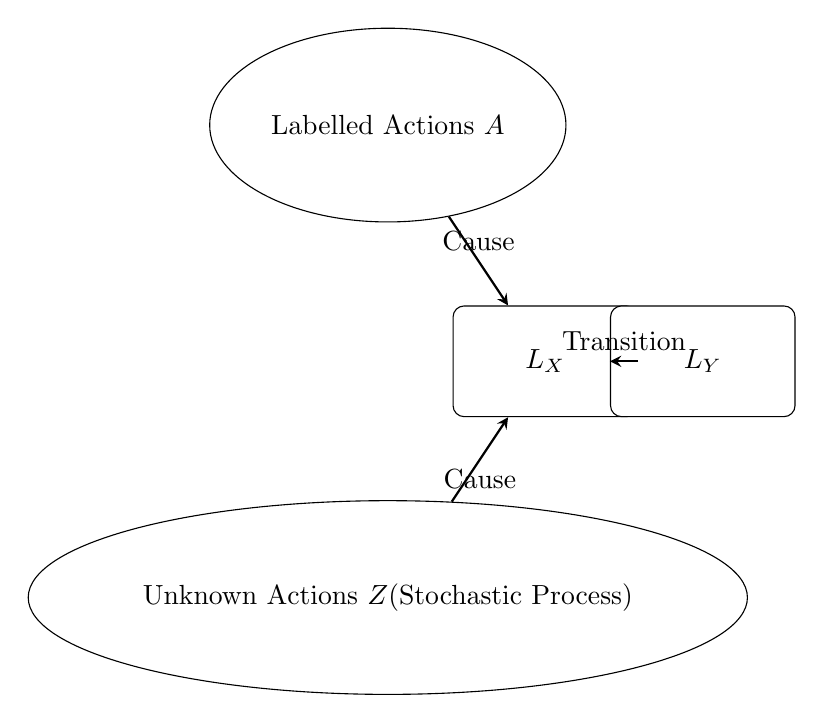
\begin{tikzpicture}[node distance=2cm]

\node (LX) [block] {\( L_X \)};
\node (LY) [block, right of=LX] {\( L_Y \)};
\node (A) [cloud, above of=LX, xshift=-2cm] {Labelled Actions \( A \)};
\node (Z) [cloud, below of=LX, xshift=-2cm] {Unknown Actions \( Z \) \\ (Stochastic Process)};

% Draw lines
\draw [line] (A) -- node[above] {Cause} (LX);
\draw [line] (Z) -- node[below] {Cause} (LX);
\draw [line] (LX) -- node[above] {Transition} (LY);

\end{tikzpicture}
\end{document}